\subsection{Heat-kernel coefficient map and local spectral-scale bifurcation}

The local target action is written as
\begin{equation}
\label{eq:chi-effective-action}
\begin{aligned}
\Gammaeff
=
\int d^4x\sqrt{-g}\,
\Big[
c_R\chigeo^2R
+Z_\chi(\partial\chigeo)^2
-\mu_\Phi^2(\chigeo)\,\Phi^\dagger\Phi
+\lambda_\Phi(\Phi^\dagger\Phi)^2
+\frac{1}{6M^2}R^2
+\cdots
\Big].
\end{aligned}
\end{equation}
The relative bosonic endomorphism used below is
\begin{equation}
\label{eq:relative-bosonic-endomorphism}
E_{\mathrm{rel}}
=
-\frac14 R\,\mathbf 1_{48}
-
(\Phi^\dagger\Phi)\,P_2
+
\frac12\gamma^{\mu\nu}\mathbb F_{\mu\nu},
\end{equation}
and the coefficient bookkeeping expected from the relative spectral expansion is summarized in \Cref{tab:heat-kernel-map}.

\begin{table}[t]
\centering
\small
\begin{tabularx}{\linewidth}{@{}>{\raggedright\arraybackslash}p{0.15\linewidth}>{\raggedright\arraybackslash}p{0.22\linewidth}>{\raggedright\arraybackslash}p{0.22\linewidth}>{\raggedright\arraybackslash}p{0.14\linewidth}>{\raggedright\arraybackslash}p{0.14\linewidth}@{}}
\toprule
Coefficient & Operator sector & Generated term & $\chigeo$ scaling & Status \\
\midrule
$a_0$ & relative bulk trace & vacuum-energy bookkeeping & $\chigeo^4$ & Hard \\
$a_2$ & seam-even bosonic bulk term & $\chigeo^2R$, $\chigeo^2\Phi^\dagger\Phi$ & $\chigeo^2$ & Closure \\
$a_4$ & local bosonic sector & $|D\Phi|^2$, $(\Phi^\dagger\Phi)^2$, $R\,\Phi^\dagger\Phi$, $\tr\mathbb F^2$, $R^2$ & $\chigeo^0$ & Closure \\
boundary/defect term & seam correction and parity data & local defect counterterms, seam-even selection & $\Delta_{\Seam}$ & Closure \\
$\eta$ term & APS spectral asymmetry & sign and spectral-flow control & scale free & Closure \\
\bottomrule
\end{tabularx}
\caption{Heat-kernel map for the geometric closure architecture.}
\label{tab:heat-kernel-map}
\end{table}

The resulting geometric logic is displayed in \Cref{fig:chi-bifurcation}. The same coefficient map controls the Einstein term, the Higgs normalization, the Higgs vacuum relation, and the curvature/gauge side terms. This is why the local spectral-scale sector is the principal geometric closure channel of the manuscript rather than just one more scalar parameter.

\begin{figure}[t]
\centering
\scriptsize
\begin{tikzpicture}[
    >=Latex,
    node distance=8mm and 11mm,
    a2/.style={draw=blue!60!black, fill=blue!6, rounded corners, align=center, text width=2.2cm, minimum height=0.9cm},
    a4/.style={draw=purple!70!black, fill=purple!7, rounded corners, align=center, text width=2.2cm, minimum height=0.9cm},
    flow/.style={draw=orange!75!black, fill=orange!8, rounded corners, align=center, text width=2.35cm, minimum height=0.95cm},
    outbox/.style={draw=green!50!black, fill=green!8, rounded corners, align=center, text width=2.6cm, minimum height=0.95cm}
]
\node[a2] (a2node) {$a_2^{\mathrm{rel}}$\\mass-scale terms};
\node[a4, right=24mm of a2node] (a4node) {$a_4^{\mathrm{rel}}$\\kinetic / quartic / curvature terms};

\node[flow, below=of a2node] (ein0) {$\chigeo^2R$\\Einstein seed};
\node[flow, below=of a4node] (kin0) {$|D\Phi|^2,\ (\Phi^\dagger\Phi)^2$\\$\tr\mathbb F^2,\ R^2$};
\node[flow, below=of $(ein0)!0.5!(kin0)$, yshift=-3mm] (chi) {same seam-even $\chigeo$ channel\\relative coefficient map};

\node[outbox, below left=of chi] (mpl) {$\Mpl^2=\chigeozero^2/(2\pi^2)$\\Einstein branch};
\node[outbox, below=of chi] (zh) {$Z_H=1/(16\pi^2)$\\canonical Higgs normalization};
\node[outbox, below right=of chi] (vev) {$\vgeo^2=Z_H\,\mu_\Phi^2(\chigeozero)/\lambda_\Phi$\\Higgs vacuum branch};
\node[flow, right=18mm of vev] (curv) {$R^2/M^2,\ \tr\mathbb F^2$\\higher-curvature / gauge branch};

\draw[->, thick] (a2node) -- (ein0);
\draw[->, thick] (a4node) -- (kin0);
\draw[->, thick] (ein0) -- (chi);
\draw[->, thick] (kin0) -- (chi);
\draw[->, thick] (chi) -- (mpl);
\draw[->, thick] (chi) -- (zh);
\draw[->, thick] (chi) -- (vev);
\draw[->, thick] (kin0.east) -- (curv.west);
\draw[->, thick] (zh) -- (vev);
\end{tikzpicture}
\caption{Coefficient flow of the local spectral-scale channel. The $a_2$ coefficient supplies the Einstein and Higgs mass seeds, the $a_4$ coefficient supplies kinetic/quartic/gauge-curvature data, and the same seam-even $\chigeo$ response turns both streams into the coupled relations for $\Mpl$ and $\vgeo$.}
\label{fig:chi-bifurcation}
\end{figure}

\begin{proposition}[Canonical bosonic normalization on the seam-even branch]
\label{prop:canonical-bosonic-normalization}
On the seam-even bosonic branch selected by $P_2$, the relative Seeley--DeWitt map is
\begin{equation}
\label{eq:relative-a2}
\begin{aligned}
a_2^{\mathrm{rel}}
=
-\int d^4x\sqrt g
\left(
\frac{\chigeo^2}{4\pi^2}R
+
\frac{\chigeo^2}{8\pi^2}\Phi^\dagger\Phi
\right)
+
a_{2,\Seam},
\end{aligned}
\end{equation}
\begin{equation}
\label{eq:relative-a4}
\begin{aligned}
a_{4,\mathrm{rel}}
=
\int d^4x\sqrt g
\left[
\frac{1}{16\pi^2}|D\Phi|^2
+
\frac{1}{16\pi^2}(\Phi^\dagger\Phi)^2
+
\frac{1}{96\pi^2}R\,\Phi^\dagger\Phi
+
\frac{1}{192\pi^2}\tr\mathbb F^2
+\dots
\right]
+
a_{4,\Seam}.
\end{aligned}
\end{equation}
Therefore the bosonic normalization constants are
\[
\Mpl^2=\frac{\chigeozero^2}{2\pi^2},
\qquad
Z_H=\frac{1}{16\pi^2},
\qquad
\Phi_{\mathrm{can}}:=\sqrt{Z_H}\,\Phi=\frac{\Phi}{4\pi},
\]
and the canonical Higgs vacuum relation becomes
\begin{equation}
\label{eq:induced-einstein}
\Mpl^2=\frac{\chigeozero^2}{2\pi^2},
\qquad
\vgeo^2=Z_H\,\frac{\mu_\Phi^2(\chigeozero)}{\lambda_\Phi}.
\end{equation}
\end{proposition}

\begin{proof}[Proof sketch]
The operator \Cref{eq:relative-bosonic-endomorphism} is the seam-even bosonic endomorphism entering the relative heat-kernel expansion. The $a_2$ coefficient fixes the Einstein branch and the bosonic mass term, while $a_4$ fixes the scalar kinetic normalization, quartic coefficient, mixed curvature term, and gauge curvature trace. The coefficient of $|D\Phi|^2$ is therefore the wave-function factor $Z_H=1/(16\pi^2)$. After the canonical rescaling $\Phi_{\mathrm{can}}=\sqrt{Z_H}\,\Phi$, the Einstein and Higgs branches are read from the same relative coefficient map rather than from separate normalization conventions.
\end{proof}

\begin{remark}[Newton form is not an independent output]
Using the standard reduced-Planck definition $\Mpl^{-2}=8\pi G_N$, the first relation in \Cref{eq:induced-einstein} is equivalently
\[
G_N\chigeozero^2=\frac{\pi}{4}.
\]
This Newton-form equation is therefore a rewriting of the Einstein-branch closure, not a second independent prediction.
\end{remark}

\begin{lemma}[Two-sheet seam-even zero-mode normalization]
\label{lem:two-sheet-zero-mode-normalization}
If the seam-even Higgs zero mode is normalized across both sheets of the oriented double cover, then its branch weight is
\[
w_H
=
2\,\gcar\,\beta_{\mathrm{rad}}^2
\exp\!\left[-\frac{\alpha^{-1}(0)+\delta_{\mathrm{ph}}}{5}\right].
\]
With
\[
\mu_\Phi^2(\chigeozero)=\frac{\chigeozero^2}{8\pi^2}w_H^2,
\qquad
\lambda_\Phi=\frac{1}{16\pi^2},
\]
the canonical Higgs vacuum expectation value is
\begin{equation}
\label{eq:carrier-dressed-v}
\vgeo
=
\Mpl\,\gcar\,\beta_{\mathrm{rad}}^2\,
\exp\!\left[-\frac{\alpha^{-1}(0)+\delta_{\mathrm{ph}}}{5}\right].
\end{equation}
\end{lemma}

\begin{proof}[Proof sketch]
The two-sheet seam-even normalization doubles the unnormalized zero-mode weight and therefore produces the stated $w_H$. Since the canonical Higgs field is $\Phi_{\mathrm{can}}=\sqrt{Z_H}\,\Phi$, its vacuum relation is
\[
\vgeo^2=\frac{Z_H\mu_\Phi^2(\chigeozero)}{\lambda_\Phi}
=
\frac{\chigeozero^2}{8\pi^2}w_H^2.
\]
Using $\Mpl^2=\chigeozero^2/(2\pi^2)$ from \Cref{prop:canonical-bosonic-normalization} gives $\vgeo=\Mpl w_H/2$, hence \Cref{eq:carrier-dressed-v}.
\end{proof}

\begin{remark}[Geometric versus benchmark electroweak scales]
For source formulas driven by the bosonic closure we write $\vgeo$ for the quantity in \Cref{eq:carrier-dressed-v}. Numerically,
\[
\vgeo\approx\num{241.87}\;\mathrm{GeV}.
\]
This is the internal geometric branch value used in the charged-lepton and seesaw source formulas. When the manuscript compares to the measured electroweak vacuum parameter at the benchmark interface, it instead uses
\[
\vewref:=\num{246.22}\;\mathrm{GeV},
\]
as an external reference value. These two numbers therefore belong to different bookkeeping layers and must not be silently interchanged inside one derivation or one table.
\end{remark}

\begin{remark}[Sector-dressed local spectral-scale channels]
The quantity $\chigeozero$ entering the induced Einstein channel is not identified with the transport-sector confinement scale. In the hadronic sector we write $\chi_{\QCD}$ and regard it as a locally dressed channel obtained from the same underlying primitive response $\chiseed$ after sector-dependent renormalization and confinement-scale matching:
\[
\chiseed \longrightarrow \chigeozero \quad \text{(gravitational background)},
\qquad
\chiseed \longrightarrow \chi_{\QCD} \quad \text{(transport-dressed local channel)}.
\]
This is the minimal statement needed to avoid the otherwise immediate scale clash between the Planck bridge and the QCD string tension.
\end{remark}

\begin{figure}[t]
\centering
\scriptsize
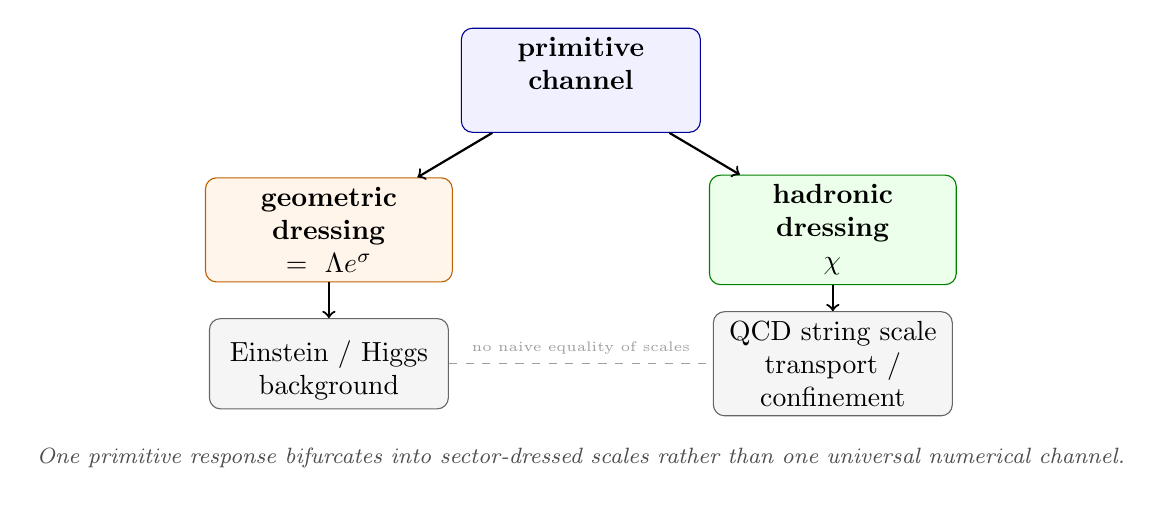
\begin{tikzpicture}[
    seed/.style={draw=blue!60!black, fill=blue!6, rounded corners, text width=2.8cm, minimum height=1.0cm, align=center},
    geo/.style={draw=orange!75!black, fill=orange!8, rounded corners, text width=2.9cm, minimum height=1.0cm, align=center},
    qcd/.style={draw=green!50!black, fill=green!8, rounded corners, text width=2.9cm, minimum height=1.0cm, align=center},
    result/.style={draw=black!60, fill=gray!8, rounded corners, text width=2.8cm, minimum height=0.95cm, align=center},
    note/.style={font=\footnotesize\itshape, text=black!70, align=center}
]
\node[seed] (seed) at (0,0) {\textbf{primitive channel}\\$\chiseed$};
\node[geo] (geo) at (-3.2,-1.9) {\textbf{geometric dressing}\\$\chigeo=\Lambda e^\sigma$};
\node[result] (geoz) at (-3.2,-3.6) {$\chigeozero$\\Einstein / Higgs background};
\node[qcd] (qcd) at (3.2,-1.9) {\textbf{hadronic dressing}\\$\chi_{\QCD}$};
\node[result] (had) at (3.2,-3.6) {QCD string scale\\transport / confinement};
\draw[->, thick] (seed) -- (geo);
\draw[->, thick] (geo) -- (geoz);
\draw[->, thick] (seed) -- (qcd);
\draw[->, thick] (qcd) -- (had);
\draw[dashed, gray!75] (geoz) -- node[above, sloped] {\tiny no naive equality of scales} (had);
\node[note] at (0,-4.8) {One primitive response bifurcates into sector-dressed scales rather than one universal numerical channel.};
\end{tikzpicture}
\caption{Local spectral-scale bifurcation. The primitive response $\chiseed$ is later dressed geometrically into $\chigeo$ and its vacuum branch $\chigeozero$, while the hadronic sector dresses the same primitive channel into $\chi_{\QCD}$. This is the clean separation that prevents the Planck/Higgs/QCD scale clash.}
\label{fig:chi-bifurcation-clean}
\end{figure}

\begin{theorem}[Relative spectral gravity branch]
\label{thm:gravity-cosmology-closure}
The same geometric closure sector defines a local spectral gravity branch of schematic form
\[
\Gamma_{\mathrm{grav}}
:=
\int d^4x\sqrt{-g}\Big[
\frac12 Z_N(\chigeo)\chigeo^2R
+\frac12 Z_\chi(\nabla\chigeo)^2
-U(\chigeo)
+R\,\mathcal F_R(\Box/\chigeo^2)R
+C\,\mathcal F_C(\Box/\chigeo^2)C
+|D\Phi|^2
-V(\Phi,\chigeo)
-\sum_a \frac{1}{4g_a^2}\tr F_{a,\mu\nu}F_a^{\mu\nu}
+\cdots
\Big].
\]
On the low-curvature local branch, the form factors reduce to the retained local coefficients and one recovers the effective action
\[
\Gamma_{\mathrm{grav}}^{\mathrm{eff}}
:=
\int d^4x\sqrt{-g}\Big[
\frac{\Mpl^2}{2}R
-\Lambda_{\Seam,\mathrm{ren}}
+\frac{1}{6M^2}R^2
+\frac{Z_\chi}{2}(\nabla\chigeo)^2
-U(\chigeo)
+|D\Phi|^2
-V(\Phi,\chigeo)
-\sum_a \frac{1}{4g_a^2}\tr F_{a,\mu\nu}F_a^{\mu\nu}
\Big],
\]
with
\[
\Mpl^2=\frac{\chigeozero^2}{2\pi^2},
\qquad
\vgeo^2=\frac{Z_H\mu_\Phi^2(\chigeozero)}{\lambda_\Phi}.
\]
Its low-curvature Euler--Lagrange equations are
\[
\Mpl^2 G_{\mu\nu}
+\Lambda_{\Seam,\mathrm{ren}} g_{\mu\nu}
+\frac{1}{3M^2}\mathcal H_{\mu\nu}
=
T_{\mu\nu}^{(\chigeo,\Phi,A,\psi)},
\]
\[
Z_\chi\Box\chigeo=U'(\chigeo)+\partial_{\chigeo}V(\Phi,\chigeo),
\qquad
D^\mu D_\mu\Phi=\partial_{\Phi^\dagger}V(\Phi,\chigeo),
\]
where
\[
\mathcal H_{\mu\nu}
:=
RR_{\mu\nu}
-\frac14 g_{\mu\nu}R^2
-\nabla_\mu\nabla_\nu R
+g_{\mu\nu}\Box R.
\]
On the low-curvature vacuum branch
\[
R\ll M^2,
\qquad
\chigeo=\chigeozero,
\qquad
\Phi=\frac{1}{\sqrt2}\binom{0}{\vgeo},
\]
the theory reduces to Einstein gravity with renormalized seam vacuum energy $\Lambda_{\Seam,\mathrm{ren}}$.
On the early-universe $R^2$ branch, the Einstein-frame scalaron potential is
\[
V_{\mathrm{sc}}(\varphi)
=
\frac34 M^2\Mpl^2
\left(1-e^{-\sqrt{2/3}\,\varphi/\Mpl}\right)^2
+\Lambda_{\Seam,\mathrm{ren}}.
\]
For spatially flat FRW one has
\[
3\Mpl^2\Hhub^2
=
\frac12\dot\varphi^2+V_{\mathrm{sc}}(\varphi)+\rho_m,
\qquad
\dot{\Hhub}
=
-\frac{1}{2\Mpl^2}\bigl(\dot\varphi^2+\rho_m+p_m\bigr),
\]
and the usual slow-roll observables
\[
A_s=\frac{V_*}{24\pi^2\Mpl^4\epsilon_*},
\qquad
n_s=1-6\epsilon_*+2\eta_*,
\qquad
r=16\epsilon_*.
\]
\end{theorem}

\begin{proof}[Proof sketch]
The $a_2$ and $a_4$ coefficient map of \Cref{eq:chi-effective-action,eq:relative-a2,eq:relative-a4}, together with the local spectral-scale formulation of \Cref{def:local-spectral-scale}, already contains the Einstein term, the Higgs sector, the $R^2$ branch, and the gauge-curvature sector in one seam-even closure package. The low-curvature limit freezes $\chigeo$ and $\Phi$ on the vacuum branch, while the higher-curvature terms reduce to the retained local $R^2$ approximation used here.
\end{proof}

\begin{corollary}[Classical limit]
On the vacuum branch the effective theory reproduces Einstein gravity with cosmological constant, Standard Model gauge fields, one seam-even Higgs doublet, and three chiral families.
\end{corollary}

\begin{conjecture}[UV program and completion criteria]
The present local gravity branch is the infrared face of a carrier-compatible
nonlocal UV completion on an admissible Bernstein form-factor cone. The effective
average action is sought in the form
\[
\Gamma_k
=
\int d^4x\sqrt g\,
\Bigl[
\frac{M_k^2}{2}R
+C\,\mathcal F_{C,k}(\Box/\chigeo^2)\,C
+R\,\mathcal F_{R,k}(\Box/\chigeo^2)\,R
+\frac12 Z_{\chi,k}(\nabla\chigeo)^2
+U_k(\chigeo,\Phi)
+\cdots
\Bigr],
\]
where the sector form factors are constrained by complete Bernstein functions
\[
\Phi_{s,k}(z)
:=
a_{s,k}+b_{s,k}z+\int_0^\infty \frac{z}{u+z}\rho_{s,k}(u)\,du,
\qquad
\rho_{s,k}(u)\ge 0.
\]
The admissible RG flow is required to preserve both the retained sector and this
cone:
\[
\partial_t\Gamma_k
:=
\frac12\mathrm{STr}_{\Padm}
\Bigl[
\bigl(\Gamma_k^{(2)}+R_k\bigr)^{-1}\partial_t R_k
\Bigr],
\]
with regulator $R_k$ commuting with $\Padm$, $Q_\Theta$, and $\inv$ and living in
the same Bernstein class. Sectorwise the inverse propagators are then required to
take the form
\[
\Gamma^{(2)}_{2,k}(p^2)
=
Z_{N,k}\,p^2\,\Phi_{2,k}(p^2/\chigeo^2),
\]
\[
\Gamma^{(2)}_{0,k}(p^2)
=
Z_{0,k}\,(p^2+M_{s,k}^2)\,\Phi_{0,k}(p^2/\chigeo^2).
\]
A genuine UV completion is reached only if three conditions close
simultaneously:
\begin{enumerate}[label=(\roman*), leftmargin=1.5em, topsep=3pt, itemsep=2pt]
    \item the admissible Bernstein cone is invariant under the projected RG flow,
    \item the flow admits a nontrivial UV fixed point on that cone,
    \item and the pole/positivity audit closes on $\operatorname{Ran}(\Padm)$:
    exactly one massless spin-$2$ pole, exactly one healthy scalaron pole with
    $M_{s,k}^2>0$ and positive residue, no extra ghost/tachyon branches, and
    positive spectral density compatible with admissible reflection positivity.
\end{enumerate}
Before these conditions are met, the manuscript treats the UV story as a
program rather than as a proved completion theorem.
\end{conjecture}

\begin{remark}[Moment-body route to the UV fixed point]
A workable proof strategy is to project the positive densities $\rho_{s,k}$ to a
compact moment body on which the RG map acts continuously and invariantly. In
that reduced picture a Schauder-type fixed-point argument becomes plausible,
while the large-$z$ asymptotics of the Bernstein functions controls the number of
relevant UV directions. This is the cleanest current route from the semiclassical
branch to a real UV completion theorem.
\end{remark}

The E$_8$ scale ladder is not used as a primitive input in the main text. Only its short downstream grammar is retained in the dedicated main-text section, while the fuller arithmetic continuations are deferred to Appendix~\ref{app:constants}.

